\documentclass[a4paper]{report}

\author{Misrraim~Su\'arez~P\'erez}
\title{FirstMarket}

\linespread{1.25}

\usepackage{comment}
\usepackage[utf8]{inputenc}

\usepackage{csquotes}

\usepackage{graphicx}
\graphicspath{ {./images/} }

\usepackage{xcolor}

\usepackage{listings}
\lstdefinelanguage{JavaScript}{
	keywords={typeof, new, true, false, catch, function, return, null, catch, switch, var, if, in, while, do, else, case, break, let, const},
	keywordstyle=\color{blue}\bfseries,
	ndkeywords={class, export, boolean, throw, implements, import, this},
	ndkeywordstyle=\color{darkgray}\bfseries,
	identifierstyle=\color{black},
	sensitive=false,
	comment=[l]{//},
	morecomment=[s]{/*}{*/},
	commentstyle=\color{purple}\ttfamily,
	stringstyle=\color{olive}\ttfamily,
	morestring=[b]',
	morestring=[b]"
}
\lstset{
	language=JavaScript,
	backgroundcolor=\color{lightgray},
	extendedchars=true,
	basicstyle=\footnotesize\ttfamily,
	showstringspaces=false,
	showspaces=false,
	numbers=left,
	numberstyle=\footnotesize,
	numbersep=9pt,
	tabsize=2,
	breaklines=true,
	showtabs=false,
	captionpos=b
}



\begin{document}

    \maketitle
    \tableofcontents

    % INTRODUCCION
    \section{Introducción}
    El presente proyecto se enmarca dentro del Proyecto Final de Grado correspondiente al Grado en Ingeniería Informática de la Universidad Nacional de Educación a Distancia.
    \\
    
    Se basa en el proyecto específico ofertado por el Departamento de Sistemas de Comunicación y Control de la UNED titulado \emph{Desarrollo de un portal de comercio electrónico}. Citando la propia descripción de dicha oferta de proyecto específico:
    
    \begin{displayquote}
        El proyecto consiste en el desarrollo de un portal web orientado al comercio electrónico.
        Dicha aplicación permitirá al comprador seleccionar artículos, realizar pedidos y pagos a través de una pasarela.
        El sistema también ofrecerá al comerciante gestionar los artículos expuestos en el portal.
    \end{displayquote}

	En este contexto, el comercio electrónico desarrollado a sido una librería, denominada \textbf{FirstMarket}.

    \subsection{Motivación y Objetivos}
    Desde un primer momento la intención fue desarrollar un proyecto que tuviese la mayor proyección posible en el mercado laboral, lo que, junto con un fuerte interés personal hacia el ecosistema de internet, llevó a la decisión de escoger esta propuesta.
    \\
    
    La idea era desarrollar algo moderno, útil, con reflejo real en la sociedad y que, como se ha dicho, cumpliese el papel de facilitar la inserción laboral. En este sentido, las aplicaciones web en general, y las específicas de comercio electrónico en particular, cumplen a la perfección los requisitos comentados. A nadie se le escapa hoy en día la implantación casi ubicua que estas tecnologías tienen en la sociedad.
    \\

    Por otro lado, y en clara conexión con lo comentado, otro objetivo de este último trabajo del plan de estudios fue el de servir como \emph{compensador} final de carencias formativas. En este sentido, el control de versiones con Git era una tarea pendiente inaplazable, así como profundizar en tecnologías web básicas como HTTP, HTML, CSS ó JavaScript. Además, ampliar el dominio de las tecnologías Java siempre fue algo muy deseable.
    \\

    Conviene no dejar de lado, por obvio, que un objetivo fundamental del presente trabajo es el de dar fin al plan de estudios. Remarcar esto es relevante porque en múltiples situaciones puede entrar en conflicto con la intención de desarrollar una aplicación web lo más moderna posible. Como se explicará más adelante en esta memoria, el mundo de las tecnologías web es muy cambiante, y pretender desarrollar una aplicación web alineada con el estado del arte en la materia partiendo, como es el caso, desde prácticamente cero conocimientos, sale fuera del marco de un trabajo de estas características. Por tanto, siempre se ha tenido en cuenta un compromiso entre recursos disponibles (principalmente tiempo y conocimientos) y grado de modernidad en las tecnologías usadas.
    \\
    
    En definitiva, el principio fundamental que ha guiado la toma de decisión ha sido el reforzar, y alinear en la medida de lo posible con el estado del arte,las habilidades técnicas fruto del plan de estudios, de forma a facilitar una futura integración en la industria web, a la par de satisfacer una histórica inquietud personal en la materia.


    \subsection{Internet, Web y Aplicaciones Web}
    En esta sección se ofrece una introducción, meramente descriptiva, del contexto en el que situar la aplicación web desarrollada. Se tratará de diferenciar los conceptos de Internet, World Wide Web y aplicaciones web.

    \subsubsection{¿Qué es Internet?}
    Tal como se explica en [computer-networking], esta pregunta puede ser enfocada desde dos puntos de vista complementarios.
    \\

    Por un lado, desde una perspectiva \textbf{hardware}, Internet es una red que conecta miles de millones de dispositivos en todo el mundo, denominados \emph{hosts} o \emph{sistemas finales}, por medio de \emph{enlaces de comunicación} y \emph{conmutadores de paquetes}.
    \\
    
    Los enlaces de comunicación son diferentes tipos de medios físicos a través de los cuales se transfieren ondas electromagnéticas que portan la información. Puede tratarse de medios guiados, como cables de cobre, cables coaxiales o fibra óptica, o no guiados, como el espectro de radio. Cuando un sistema final decide enviar información a otro sistema final, el emisor fragmenta los datos en \emph{paquetes} de información y los envía al destinatario a través de la red. Una vez en destino, el sistema final receptor ensambla los paquetes para reconstruir los datos originales. Un conmutador de paquetes toma un paquete que llega a uno de sus enlaces de comunicación entrantes y decide hacia cuál de sus enlaces de comunicación salientes lo reenvía.
    \\

    Estas \emph{redes de conmutación de paquetes} se pueden entender de forma análoga a una empresa que necesita mover una gran cantidad de carga entre dos almacenes separados gran distancia. En el almacén de origen la carga se divide y organiza en diferentes contenedores. Cada uno de los contenedores viaja de forma independiente a través de la red de transporte disponible siguiendo posiblemente rutas no del todo iguales. Por ejemplo, unos contenedores pueden ir por ciertas carreteras en ciertos camiones mientras que otros pueden viajar en tren o incluso en barco, o cualquier combinación de los anteriores. Lo importante es la independencia entre la ruta de un contenedor concreto con los demás. Una vez llegados al almacén de destino, la carga se extrae de los contenedores y se agrupa con el resto que llega del mismo envío. Así, los paquetes son análogos a los contenedores, los enlaces de comunicación son análogos a las vías de transporte, los conmutadores de paquetes son análogos a las intersecciones o discontinuidades en las vías de transporte (piénsese en una simple rotonda), y los sistemas finales son análogos a los almacenes. Pues bien, de igual forma que un contenedor toma un camino a través de la red de transporte, un paquete de información toma un camino a través de la infraestructura de Internet.
    \\

    Por otro lado, es posible describir Internet desde un punto de vista \textbf{software} como un servicio prestado a las aplicaciones distribuidas, es decir, como una interfaz de programación que las aplicaciones distribuidas consumen.
    \\
    
    Se dice que las aplicaciones son aplicaciones distribuidas, o \textbf{aplicaciones de Internet}, cuando se ejecutan en diferentes máquinas que intercambian datos entre sí. Es importante destacar que las aplicaciones de Internet se ejecutan estrictamente en los sistemas finales, no en la infraestructura de la red, que es agnóstica (o debiera serlo) de la semántica de la información que está trasportando. Así, puede pensarse en Internet como un servicio postal, que garantiza el envío de información entre partes, las cuales pueden estar desarrollando cualquier tipo de actividad basada, entre otras cosas, en la propia comunicación que mantienen. Al igual que el servicio postal impone una serie de reglas para ser usado, como dónde depositar la carta que se pretende enviar o dónde y de qué manera especificar la dirección de envío, Internet ofrece unas reglas en forma de interfaz de programación que las aplicaciones de Internet deben adoptar.
    
    \subsubsection{¿Qué es la Web?}
    Siguiendo el hilo de la discusión del epígrafe anterior, la World Wide Web es una de las muchas aplicaciones de Internet existentes. Otras serían el correo electrónico, las aplicaciones para acceder remotamente a otra máquina, la transferencia de archivos, el streaming de video, la telefonía por Internet, y más.
    \\
    
    A veces, dado que la Web es la aplicación más conocida, se confunde la parte con el todo al identificarla con la propia Internet. Sin embargo, esta aplicación surgió bastante tiempo después de que otras ya estuvieran ampliamente implantadas y maduras, como el correo electrónico o la transferencia de ficheros, si bien su uso era principalmente en ámbitos académicos.
    \\
    
    Lo que da tanta importancia a la Web es que fue la aplicación de Internet que, a principios de los años 90, abrió al gran público a la hasta entonces desconocida Internet. De hecho, esta aplicación llevó a Internet de ser tan sólo una más de muchas redes existentes a ser la dominante por excelencia.
    \\
    
    Entonces, como se ha dicho, la Web es una aplicación de Internet, y como tal se trata de software que se ejecuta en diferentes máquinas que intercambian mensajes entre sí. El formato de estos mensajes, su timing y demás \emph{reglas de conversación} se recogen en un protocolo, el HyperText Transfer Protocol (HTTP). Este protocolo es el corazón de la Web, encontrandose definido en [RFC 1945] y en [RFC 2616], y su implementación se materializa en dos programas ejecutados en diferentes sistemas finales, un programa cliente y un programa servidor.
    \\
    
    La mecánica básica gira en torno a peticiones y respuestas. El programa cliente envía un mensaje HTTP conteniendo una petición al programa servidor. Por su parte, siguiendo las reglas definidas en el protocolo, el programa servidor contesta enviando otro mensaje HTTP al cliente. En el caso más común, el cliente le solicita al servidor el envío de una \emph{página web}.
    \\
    
    Una página web es un documento de texto escrito con unas reglas de sintaxis específicas. Estas reglas definen el Hypertext Markup Language (HTML). En el sistema final cliente, la página web es presentada en pantalla de una manera amigable al usuario por medio de programas que procesan el contenido en HTML.
    \\
    
    En definitiva, y sin entrar en matices que desvíen de la esencia, la Web es la aplicación de Internet que permite el consumo de páginas web bajo demanda por parte de los usuarios (en contraste con el modelo broadcast, en el que se emite y el usuario sólo puede consumir lo emitido, como en la radio).
    
    \subsubsection{¿Qué es una Aplicación Web?}
    Las páginas web que son enviadas desde el servidor al cliente se dice que pueden ser estáticas o dinámicas. Esta característica, más que hablar de la página web en sí misma, habla del proceso mediante el cual su contenido ha sido creado y modificado a lo largo del tiempo.
    \\
    
    Las páginas estáticas lo son en el sentido de que su contenido, creado comunmente por un humano, no varía con el tiempo de manera programática. La información que presentan es la misma, a menos que se modifique \emph{a mano}. Así eran todas las páginas web en los primeros años. En contraste, en las páginas web dinámicas, el contenido no está dado de antemano, sino que se genera en cada ciclo de petición-respuesta. Esto es útil porque entre otras cosas permite páginas web personalizadas para cada usuario, e incluso que sea él mismo quien aporte contenido a la página web.
    \\
    
    Una \textbf{aplicación web} es el sistema software encargado de la generación dinámica de páginas webs. Normalmente, y a diferencia del modelo estático, entre sus componentes se encuentra una base de datos que permita la persistencia de la información, cambiante por definición de la propia arquitectura.
    \\
    
    Desde este punto de vista, en el presente proyecto se ha desarrollado una aplicación web encargada de generar contenido web que los usuarios pueden visitar con el objetivo de comprar libros a través de Internet.

    \subsection{Estructura de la Memoria}
    Estructura

    % ANALISIS
    \section{Análisis}

        \subsection{Requisitos}

            La aplicación debe admitir los roles y capacidades siguientes:
            \begin{enumerate}
                \item Usuario an\'onimo (UA).
                \begin{itemize}
                    \item Por defecto, al acceder al sitio web se hace como UA, sin ninguna validacion ni credencial. Basta con acceder a la pagina (url) de inicio de la aplicacion.
                    \item Un UA debe poder realizar b\'usquedas de libros, es decir, debe tener pleno acceso a la exploracion del cat\'alogo.
                    \item La plena exploraci\'on del cat\'alogo debe permitir realizar b\'usque\-das filtradas seg\'un 0, 1 o m\'as criterios, tales como: categor\'\i{}a, t\'\i{}tulo o autor.
                    \item Un UA debe poder visualizar informacion detallada de un libro, por ejemplo de entre los obtenidos tras una busqueda.
                    \item Un UA debe poder consultar las promociones disponibles.
                    \item Un UA debe poder registrarse en el sistema completando un formulario (nombre, contrase\~na, direccion de correo electronico, etc.).
                    \item finalizado el proceso de registro, el nuevo UR debe recibir confirmacion por e-mail
                    \item en su caso, un UA debe poder hacer login en el sistema.
                    \item en su caso, un UA debe poder realizar el procedimiento de recuperacion de contrase\~na.
                \end{itemize}
                \item Usuario registrado (UR). Este perfil representa a un usuario que ha pasado de an\'onimo a registrado. Un UR posee todas las capacidades del UA, m\'as otras espec\'\i{}ficas suyas, a saber:
                \begin{itemize}
                    \item Poder editar la informacion de su perfil de usuario.
                    \item Realizar pedidos y efectuar los correspondientes pagos a traves de una pasarela segura.
                    \item Disponer de un carrito virtual para la gestion de la compra.
                    \item En el carrito se debe poder introducir, modificar la cantidad o eliminar libros (esto ultimo de uno en uno o todos a la vez).
                    \item en cualquier momento del proceso de realizar un pedido, el UR debe poder cancelarlo
                    \item Tras una compra, el UR debe recibir confirmacion en su correo electronico
                    \item un UR debe poder consultar el estado de sus pedidos
                    \item Puntuar (de alguna manera, p.e. estrellas del 1 al 5) un determinado libro que haya adquirido. Debe poder hacerlo en cualquier momento tras la compra.
                    \item Consultar un historico de sus transacciones, detallando los libros comprados, la fecha de la compra y el precio de cada uno.
                    \item Darse de baja como UR.
                    \item Cerrar sesion.
                    \item Un UR debe poder ponerse en contacto con el admin a traves de un formulario de contacto, recibiendo confirmacion por e-mail tras el envio del mismo.
                \end{itemize}
                \item Usuario Administrador
                \begin{itemize}
                    \item Ver y editar (a\~nadir, modificar, eliminar) la jerarquia de categorias (CRUD categorias).
                    \item Ver y editar (a\~nadir, modificar, eliminar) la informacion relativa a los libros (titulo, autor/es, editorial, precio, disponibilidad, \ldots) (CRUD libros).
                    \item Crear, modificar o eliminar promociones de libros (CRUD promos).
                    \item Tener acceso a la informacion de los UR, salvo sus contrase\~nas.
                    \item Dar de baja a un UR.
                    \item Visualizar la informacion de los pedidos, tanto los que esten en curso como los finalizados.
                    \item Poder alterar el estado de un pedido.
                    \item Poder generar informes (p.e. ventas durante un determinado periodo con su importe y la facturacion total).
                \end{itemize}
            \end{enumerate}

            Además de lo anterior, la aplicación debe:
            \begin{enumerate}
                \item[a)] garantizar la persistencia de los datos referentes a UR, pedidos, pagos, productos y sus categorías
                \item[b)] mostrar un mensaje de error cuando un usuario introduzca incorrectamente sus credenciales de autenticación
            \end{enumerate}

        \subsection{Casos de Uso}
            En este apartado se presenta las interacciones más comunes que los usuarios pueden realizar con la aplicación web. No se pretende proporcionar una enumeración exhaustiva de todos los casos de uso, sino un subconjunto relevante de los mismos, a modo de introducción a las capacidades básicas que se espera de la aplicación.

            \begin{figure}[h]
                \centering
                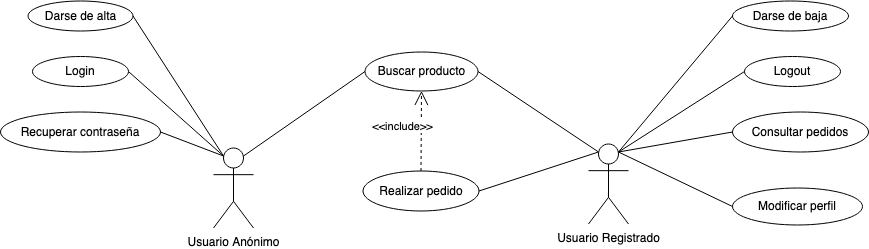
\includegraphics[width=\textwidth]{Use-Case_Diagram}
            \end{figure}

            \subsubsection{CU01\_Búsqueda}
            Proceso por el cual un usuario explora el cat\'alogo y acaba por visualizar la pagina de un libro.
            \begin{itemize}
                \item[+] Actores implicados: Usuario An\'onimo, Usuario Registrado.
                \item[+] Precondiciones: Nos encontramos en cualquiera de las p\'aginas que dan acceso al cat\'alogo.
                \item[+] Flujo principal:
                \begin{enumerate}
                    \item[1.] El usuario hace click en alguna de las categor\'\i{}as principales mostradas a modo de cat\'alogo flotante en la barra de navegacion
                    o hace click en \emph{All Books}.
                    \item[2.] El sistema muestra la p\'agina de resultados de b\'usqueda.
                    \item[3.] El usuario hace click en alguno de los productos mostrados.
                    \item[4.] El sistema muestra la p\'agina del libro.
                \end{enumerate}
                \item[+] Flujo alternativo: \emph{refinamiento\_b\'usqueda}. El usuario altera en la p\'agina de resultados alg\'un criterio de filtro.
                \begin{itemize}
                    \item[3.b.] El usuario selecciona/deselecciona alg\'un criterio de filtro de entre los mostrados en la p\'agina de resultados de b\'usqueda.
                    \item[4.b.] El sistema vuelve al punto 2 del flujo principal.
                \end{itemize}
                \item[+] Flujo alternativo: \emph{b\'usqueda\_por\_texto}. El usuario introduce una cadena de texto en el cuadro de b\'usqueda.
                \begin{itemize}
                    \item[1.b.] El usuario introduce una cadena de texto en el cuadro de b\'usqueda y hace click.
                \end{itemize}
            \end{itemize}

            \subsubsection{CU02\_Alta}
            Proceso por el cual se crea un nuevo usuario registrado.
            \begin{itemize}
                \item[+] Actores implicados: Usuario An\'onimo.
                \item[+] Flujo principal:
                \begin{enumerate}
                    \item[1.] El usuario hace click en el link de nuevo registro, disponible en la p\'agina de \emph{login}.
                    \item[2.] El sistema presenta un formulario donde introducir la direcci\'on de e-mail y la contrase\~na.
                    \item[3.] El usuario introduce y env\'\i{}a la informaci\'on pedida.
                    \item[4.] El sistema comprueba la informaci\'on proporcionada.
                    \item[5.] El sistema crea una nueva cuenta de usuario, pero la mantiene inactiva a la espera de confirmar la direcci\'on de email.
                    \item[6.] El sistema env\'\i{}a un email con un link de confirmaci\'on a la direcci\'on proporcionada, e informa al usuario por pantalla.
                    \item[7.] El usuario accede a su e-mail y hace click en el link enviado, confirmando que la direcci\'on de email es suya.
                    \item[8.] El sistema activa la cuenta de usuario.
                    \item[9.] El sistema env\'\i{}a al usuario un email de bienvenida.
                    \item[10.] El sistema redirige al usuario a la p\'agina de \emph{login}.
                \end{enumerate}
                \item[+] Flujo alternativo: \emph{usuario\_ya\_registrado}. La direcci\'on proporcionada se encuentra registrada en el sistema.
                \begin{itemize}
                    \item[5.b.] El sistema no crea una nueva cuenta de usuario.
                    Por razones de seguridad, la manera en que el sistema informa al usuario tras esta situacion es indistinguible del flujo principal,
                    de forma que no se pueda deducir que ese email ya tiene cuenta asociada en el sistema.
                \end{itemize}
                \item[+] Flujo alternativo: \emph{link\_ya\_enviado}. El sistema est\'a a la espera de la confirmacion de un link valido en esta direccion de email.
                \begin{itemize}
                    \item[5.b.] El sistema no crea una nueva cuenta de usuario. Se informa al usuario acerca de una condicion de error \-{}generica, por seguridad\- en relacion
                    con la direccion de email proporcionada, pidiendose que compruebe su direcci\'on de email.
                \end{itemize}
                \item[+] Flujo excepcional: \emph{time\_out}. El usuario no confirma su direccion de e-mail dentro de un plazo determinado.
                \begin{itemize}
                    \item[7.b.] El sistema detecta el timeout e invalida el link de confirmacion enviado. Si el usuario hace click en el link caducado se le informara de dicha condicion.
                \end{itemize}
            \end{itemize}

            \subsubsection{CU03\_Login}
                Proceso por el cual un usuario se autentica en el sistema.
                \begin{itemize}
                    \item[+] Actores implicados: Usuario An\'onimo.
                    \item[+] Flujo principal:
                    \begin{enumerate}
                        \item[1.] El usuario hace click en el link de \emph{login}, o intenta realizar alguna operaci\'on
                        que requiera autenticaci\'on (por ejemplo, a\~nadir un libro al carrito).
                        \item[2.] El sistema presenta el formulario de acceso (direcci\'on de email y la contrase\~na).
                        \item[3.] El usuario introduce y env\'\i{}a la informaci\'on pedida.
                        \item[4.] El sistema comprueba las credenciales.
                        \item[5.] El sistema redirige al usuario a la p\'agina principal.
                    \end{enumerate}
                    \item[+] Flujo alternativo: \emph{fallo\_autenticaci\'on}. El email no se encuentra registrado en el sistema, o la contrase\~na proporcionada no es correcta.
                    \begin{itemize}
                        \item[5.b.] El sistema informa al usuario acerca de un fallo gen\'erico de autenticaci\'on, de forma que,
                        por razones de seguridad, no se pueda deducir si el email proporcionado se encuentra registrado en el sistema.
                    \end{itemize}
                    \item[+] Flujo alternativo: \emph{bloqueo\_cuenta}. El usuario an\'onimo realiza, dentro de un marco de tiempo (configurable), un n\'umero de intentos (configurable) de login con contrase\~na err\'onea.
                    \begin{itemize}
                        \item[5.b.] El sistema bloquea la cuenta asociada al email para prevenir ataques por fuerza bruta.
                        \item[6.] El sistema informa al usuario por pantalla y mediante el env\'\i{}o de un email.
                        \item[7.] Pasado el tiempo de seguridad (configurable), el sistema desbloquea la cuenta del usuario.
                    \end{itemize}
                    \item[+] Post-Condiciones: El usuario pasa a tener rol de usuario registrado en el sistema.
                \end{itemize}

            \subsubsection{CU04\_RecuperarContrase\~na}
                Un usuario previamente registrado en el sistema intenta acceder al mismo, pero no recuerda su contrase\~na. El sistema intentar\'a crear una nueva contrase\~na y enviarla al e-mail del usuario.
                \begin{itemize}
                    \item[+] Actores implicados: Usuario An\'onimo.
                    \item[+] Flujo principal:
                    \begin{enumerate}
                        \item El usuario hace click en la opci\'on \emph{?`olvid\'o su contrase\~na?}.
                        \item El sistema presenta un formulario donde introducir la direcci\'on de e-mail.
                        \item El usuario introduce y env\'ia su direcci\'on de e-mail.
                        \item El sistema comprueba la direcci\'on de e-mail.
                        \item Comprobaci\'on correcta. El sistema env\'ia un e-mail con un link de confirmaci\'on a la direcci\'on proporcionada, e informa de ello al usuario por pantalla.
                        \item Link no caducado. El usuario accede a su e-mail y hace click en el link, confirmando que efectivamente la direcci\'on proporcionada es la suya.
                        \item El sistema genera una nueva contrase\~na y se la asigna al usuario.
                        \item El sistema env\'ia la nueva contrase\~na a la direcci\'on de e-mail del usuario, y le avisa de ello por pantalla.
                    \end{enumerate}
                    \item[+] Flujo alternativo: \emph{usuario\_no\_registrado}. La direccion proporcionada no se encuentra registrada en el sistema.
                    \begin{itemize}
                        \item[5.b.] El sistema no envia correo alguno pero, por razones de seguridad, desde el punto de vista del usuario este flujo alternativo es indistinguible del proncipal.
                    \end{itemize}
                    \item[+] Flujo excepcional: \emph{time\_out}. El usuario no confirma su direccion de e-mail dentro de un plazo determinado.
                    \begin{itemize}
                        \item[6.b.] El sistema detecta el timeout e invalida el link de confirmacion enviado. Si el usuario hace click en el link caducado se le informara de dicha condicion.
                    \end{itemize}
                \end{itemize}

            \subsubsection{CU05\_EditarPerfil}
                Proceso por el cual un usuario modifica alguno de los datos de su perfil personal.
                \begin{itemize}
                    \item[+] Actores implicados: Usuario Registrado.
                    \item[+] Flujo principal:
                    \begin{enumerate}
                        \item[1.] El usuario hace click en \emph{area personal}.
                        \item[2.] El sistema muestra la pagina de area personal, en donde se muestra el formulario de datos personales, rellenado con la informacion actual del usuario.
                        \item[3.] El usuario modifica los datos del formulario y lo envia al sistema.
                        \item[4.] El sistema comprueba los datos.
                        \item[5.] Comprobación correcta.El sistema actualiza la información del usuario.
                        \item[6.] El sistema muestra la pagina de inicio.
                    \end{enumerate}
                    \item[+] Flujo alternativo: \emph{error\_datos\_formulario}. Los datos proporcionados en el formulario de informacion personal no son validos.
                    \begin{itemize}
                        \item[5.b.] El sistema regresa al punto 3 del flujo principal, e informa al usuario acerca del fallo producido.
                    \end{itemize}
                    \item[+] Flujo alternativo: \emph{cancelar}. El usuario cancela el proceso de edicion de su informacion personal.
                    \begin{itemize}
                        \item[3.b.] El usuario hace click en el boton \emph{cancelar}. El sistema muestra la pagina de inicio.
                    \end{itemize}
                    \item[+] Post-Condiciones: El usuario ha alterado su informacion personal almacenada en la aplicacion.
                \end{itemize}

            \subsubsection{CU06\_RealizarPedido}
                Proceso por el cual un usuario realiza una compra a traves de la aplicacion web.
                \begin{itemize}
                    \item[+] Actores implicados: Usuario Registrado.
                    \item[+] Precondiciones: Desde cualquier pagina en la que se muestren libros (pagina de inicio, pagina de resultados de busqueda o pagina de un libro) el usuario hace click en \emph{add to cart}, para uno o mas libros.
                    \item[+] Flujo principal:
                    \begin{enumerate}
                        \item[1.] El usuario hace click en el icono del carrito.
                        \item[2.] El sistema muestra la pagina del carrito del usuario, con todos los libros contenidos en el mismo.
                        \item[3.] El usuario puede aumentar o disminuir el numero de unidades de un libro, o incluso eliminarlo por completo, y hace click en \emph{checkout}.
                        \item[4.] El sistema comprueba la disponibilidad de los libros contenidos en el carrito.
                        \item[5.] Stock suficiente. El sistema muestra la pagina de checkout, con el formulario de datos de envio y pago, y el resumen de la compra.
                        \item[6.] El usuario completa los datos de envio y de pago y hace click en \emph{Pay}.
                        \item[7.] El sistema tramita el pago.
                        \item[8.] Pago ok. El sistema registra el nuevo pedido.
                        \item[9.] El sistema confirma al usuario por pantalla y por e-mail que el pedido se ha realizado con exito.
                    \end{enumerate}
                    \item[+] Flujo alternativo: \emph{stock\_insuficiente}. No hay stock suficiente para satisfacer el contenido del carrito.
                    \begin{itemize}
                        \item[5.b.] El sistema vuelve al punto 2 del flujo principal, informando al usuario de los libros para los cuales no hay stock suficiente.
                        \item[3.b.] El usuario reduce la cantidad demandada de los libros correspondientes y hace click en \emph{checkout}.
                    \end{itemize}
                    \item[+] Flujo alternativo: \emph{error\_pago}. Error al efectuar el pago.
                    \begin{itemize}
                        \item[8.b.] El sistema vuelve al punto 5 del flujo principal, informando al usuario del problema respecto al pago.
                    \end{itemize}
                    \item[+] Flujo excepcional: \emph{libro\_eliminado}. Algun libro del carrito ya no esta disponible en el sistema.
                    \begin{itemize}
                        \item[5.b.] El sistema elimina del carrito automaticamente los libros que el administrador haya deshabilitado.
                        \item[6.b.] El sistema vuelve al punto 2 del flujo principal, informando al usuario de los libros que han sido eliminados.
                    \end{itemize}
                    \item[+] Post-Condiciones: El usuario ha efectuado un nuevo pedido.
                \end{itemize}

            \subsubsection{CU07\_ConsultarPedido}
                Proceso por el cual un usuario consulta el historial de pedidos que ha realizado.
                \begin{itemize}
                    \item[+] Actores implicados: Usuario Registrado.
                    \item[+] Flujo principal:
                    \begin{enumerate}
                        \item[1.] El usuario hace click en \emph{My Purchases} en la barra de navegacion.
                        \item[2.] El sistema muestra la pagina de los pedidos del usuario.
                        \item[3.] El usuario puede expandir-contraer la informacion mostrada relativa a un pedido.
                    \end{enumerate}
                \end{itemize}

            \subsubsection{CU08\_Baja}
                Proceso por el cual un usuario elimina su cuenta de la tienda online.
                \begin{itemize}
                    \item[+] Actores implicados: Usuario Registrado.
                    \item[+] Flujo principal:
                    \begin{enumerate}
                        \item[1.] El usuario hace click en \emph{area personal}.
                        \item[2.] El sistema muestra la pagina de area personal.
                        \item[3.] El usuario selecciona \emph{eliminar cuenta}.
                        \item[4.] El sistema muestra el formulario de eliminacion de cuenta.
                        \item[5.] El usuario completa y envia el formulario.
                        \item[6.] El sistema comprueba los datos.
                        \item[7.] Comprobacion correcta. El sistema actualiza el estado del usuario y envia un e-mail de confirmacion.
                        \item[8.] El sistema muestra la pagina de inicio.
                    \end{enumerate}
                    \item[+] Flujo alternativo: \emph{error\_datos\_formulario}. La contrase\~na proporcionada en el formulario de baja no es correcta.
                    \begin{itemize}
                        \item[7.b.] El sistema regresa al punto 4 del flujo principal, e informa al usuario acerca del fallo producido.
                    \end{itemize}
                    \item[+] Flujo alternativo: \emph{cancelar}. El usuario cancela el proceso de baja.
                    \begin{itemize}
                        \item[5.b.] El usuario cancela el proceso de baja. El sistema regresa al punto 2 del flujo principal.
                    \end{itemize}
                    \item[+] Post-Condiciones: El usuario ya no figura como dado de alta en la aplicacion.
                \end{itemize}

            \subsubsection{CU09\_Logout}
                Proceso por el cual un usuario cierra su sesi\'on en el sistema.
                \begin{itemize}
                    \item[+] Actores implicados: Usuario Registrado.
                    \item[+] Precondiciones: el usuario esta con su sesion abierta en el sistema.
                    \item[+] Flujo principal:
                    \begin{enumerate}
                        \item[1.] El usuario hace click en el link de \emph{logout}.
                        \item[2.] El sistema cierra la sesion del usuario.
                        \item[3.] El sistema muestra la pagina de inicio.
                    \end{enumerate}
                    \item[+] Post-Condiciones: El usuario ha efectuado el logout con exito.
                \end{itemize}


    % DISEÑO
    \section{Diseño}
    En este apartado se ofrece una descripción de las decisiones tomadas a nivel de diseño de la aplicación web.
    \subsection{Arquitectura del Sistema}
    Sin entrar en detalles internos, a vista de pájaro, la aplicación web ha sido construida siguiendo la arquitectura clásica de tres capas cliente-servidor-datos. Hoy en día, quizás, esta no sea la organización más vanguardista. Los términos \emph{serverless}, \emph{microservicios} o \emph{single-page-application} son los que con mayor eco resuenan en la industria web actual.
    
    \begin{figure}[h]
    	\centering
    	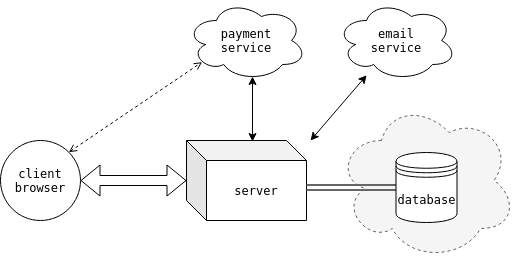
\includegraphics[width=\textwidth]{desing_diagram}
    \end{figure}
    
    Como muchas tendencias dentro del mundo de la computación, estos términos no están del todo delimitados, ofreciendo en ocasiones diferentes interpretaciones y/o solapamientos entre sí. Serverless hace mención a aquellas aplicaciones web que en su mayor parte, o por completo, incorporan servicios cloud de terceras partes para gestionar su propia lógica de negocio. La arquitectura de microservicios está muy relacionada con lo anterior, ya que esta concibe las aplicaciones como un agregado de servicios muy especializados ejecutados de forma independiente, puede que en máquinas remotas, que se comunican entre sí de manera ligera y eficiente. Por su parte, las SPA usan la elevada capacidad de cómputo de los clientes actuales para trasladar allí parte de la lógica que tradicionalmente implementa el servidor. En una SPA o bien todo el contenido HTML, JavaScript y CSS es cargado una sola vez, o bien se carga dinámicamente bajo demanda, normalmente como respuesta a las acciones del usuario, dando así una mayor sensación de fluidez.
    
    No obstante, a pesar de las muchas ventajas que presentan estas formas de enfocar las aplicaciones web, se ha optado por la arquitectura clásica (con pinceladas, como se verá, de aspectos serverless y SPA), y el motivo es doble:
    
    \begin{itemize}
    	\item[-] Antes del 2 va el 1. El punto de partida en el desarrollo de la presente aplicación web fue el de prácticamente nulos conocimientos sobre esta rama de la informática. En este escenario, antes de estudiar directamente las arquitecturas surgidas en los últimos años, se ha preferido estudiar la arquitectura clásica, en el convencimiento de que es el camino formativo correcto.
    	\item[-] Tecnología viva. En contra de lo que hace unos años algunas voces avanzaban, la arquitectura browser-server-database no está muerta y previsiblemente no lo va a estar. Esta es una tecnología madura, robusta y muy extendida. Aunque es muy cierto que su cuota de mercado ha descendido en pro de otras arquitecturas más recientes, muestra tener un suelo estable y un lugar propio dentro de las tecnologías web. En parte esto es así porque, como casi siempre, no es oro todo lo que reluce. Las arquitecturas modernas no son la perfección, mostrando tener algunos puntos débiles. Ver []
    \end{itemize}
    
    En la imagen XX se presenta un esquema de la arquitectura de la aplicación web. Como se aprecia, responde a la mencionada arquitectura clásica de tres capas cliente-servidor-datos. No obstante, existen ciertos elementos que descansan en servicios cloud externos. Este es el aspecto serverless al que se hizo mención anteriormente. Asi, el servicio de pagos es ofrecido por Stripe (ref sección stripe). Como se aprecia en la imagen XX, existe una vía de comunicación directa entre el cliente y Stripe. Esto es así para garanatizar que la aplicación web no tiene nunca acceso a los datos confidenciales de pago del cliente (p.e., número de la tarjeta de crédito), sino que esta información es enviada directamente desde el cliente a Stripe. Por su parte, el servicio de correo es delegado en Gmail, a través de la capa de abstracción que Spring Framework ofrece de la API JavaMail. Y, por último, la base de datos. Este caso es especial porque dependiendo del entorno de ejecución se puede asimilar a un servicio cloud o no. En este sentido, cuando el entorno de ejecución es producción, la base datos es accedida como un servicio que AWS presta a Heroku.
    \\
    
    Centrando la atención ahora en el núcleo de la aplicación, es decir, dejando de lado los servicios periféricos de pago y correo, el principio de diseño más relevante es la \textbf{separación de responsabilidades} (\emph{separation of concerns}, SoC). Como se muestra en la imagen YY, esto se consigue organizando funcionalmente la aplicación en capas: web, negocio y persistencia. Además, la aplicación ha sido desarrollada haciendo uso de un framework -Spring Framework [ref]- de inversión de control (\emph{inversion of control}, IoC) e inyección de dependencias (\emph{dependency injection}, DI), dos patrones de diseño sumamente importantes.
    
    \begin{figure}[h]
    	\centering
    	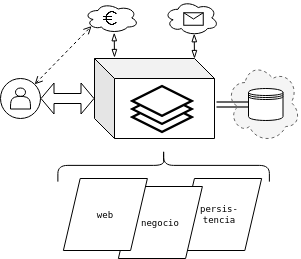
\includegraphics[width=\textwidth]{desing_layer_diagram}
    \end{figure}
    
    \subsubsection{Separación de Responsabilidades}
    \subsubsection{Inversión de Control. Inyección de Dependencias}
    
    \subsection{Modelo de Datos}
    Modelo

    % IMPLEMENTACION
    \section{Implementación}
    La implementacion del analisis y diseno detallados en los puntos anteriores lo conforma el conjunto de programas que se incluyen en el CD distribuido con la presente memoria. No obstante, en este apartado se ha querido comentar ciertos aspectos relevantes, que por la dificultad presentada y/o por el papel clave dentro de la aplicación merecen mención especial.
    
    \subsection{Control de Concurrencia}
    Uno de los aspectos más críticos para el correcto funcionamiento de una tienda online es el control del stock de productos y del proceso de realización de una compra. Muchos usuarios, quizás simultáneamente, pueden añadir productos a sus carritos y proceder a su compra. La aplicación debe garantizar que estas acciones se realicen de forma a conservar en todo momento la consistencia de los datos.
    \\
    
    \begin{figure}[hbt!]
    	\centering
    	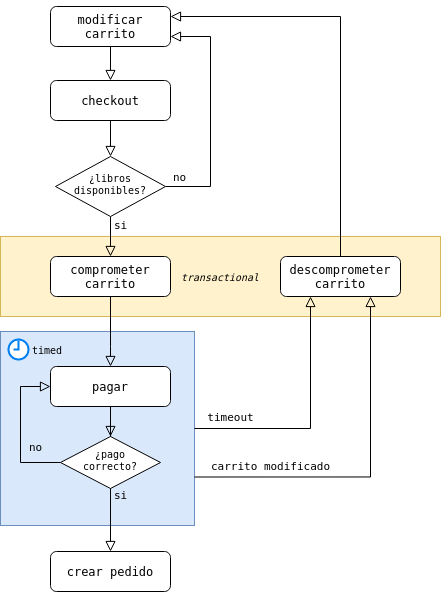
\includegraphics[width=\textwidth]{cart_diagram}
    \end{figure}
    
    Como se puede apreciar en la imagen X, cuando un usuario decide proceder con el pedido de los libros contenidos en su carrito, lo primero que hace el sistema es comprobar que esos libros están disponibles. Pueden no estarlo por dos motivos, a saber, que estén agotados en ese momento o que el administrador de la aplicación web los haya desabilitado (además, en este último caso el sistema automáticamente retira del carrito dichos libros al detectar la situación). Si alguno de estos escenarios ocurriese la aplicación informaría al usuario en la propia vista del carrito, sin avanzar a la vista de checkout, tal como se muestra en la imagen X.
    \\
    
    \begin{figure}[hbt!]
    	\centering
    	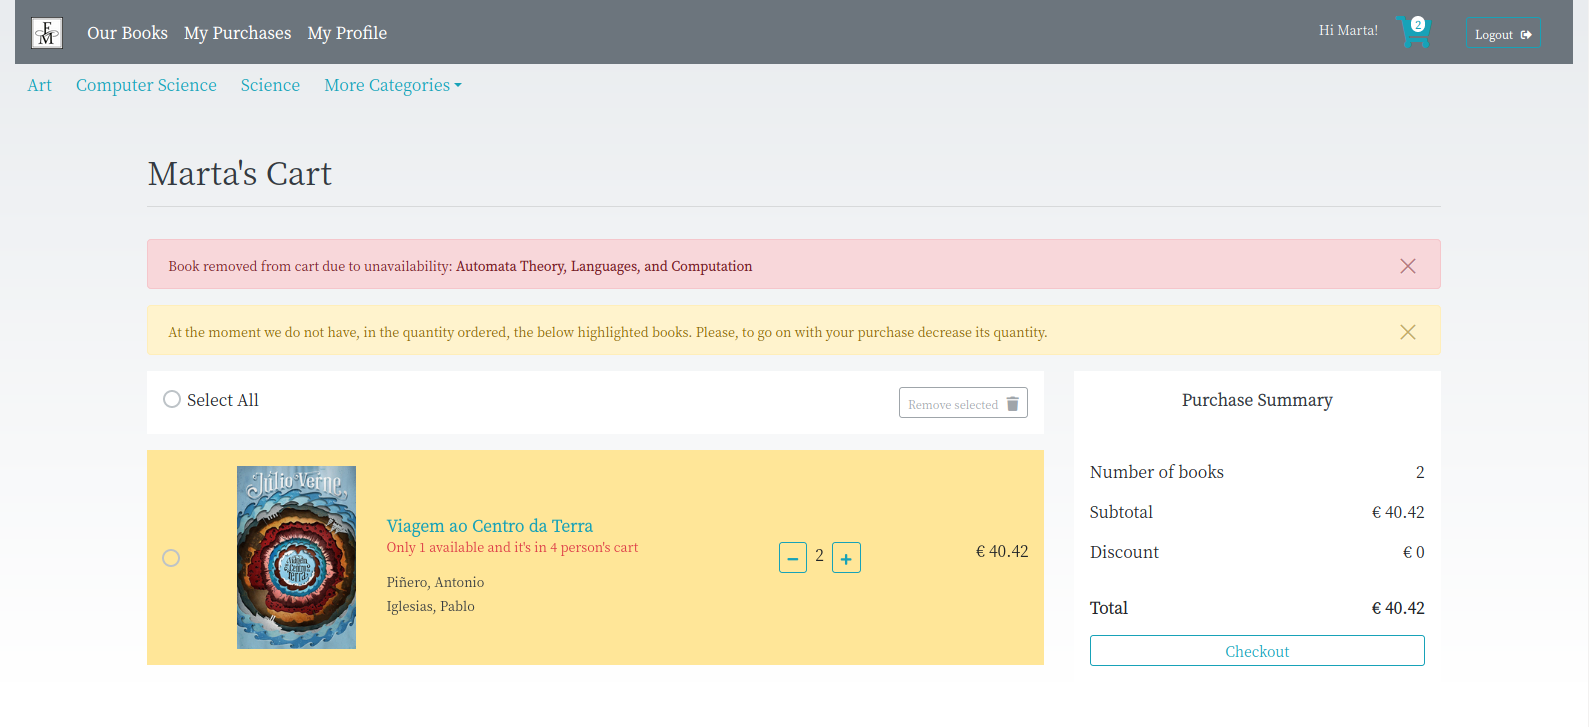
\includegraphics[width=\textwidth]{cart_alert}
    \end{figure}
    
    Tras comprobar que los libros están disponibles el sistema \textbf{compromete} el carrito. Este es el paso fundamental donde se garantiza la consistencia. El sistema se compromete con el usuario a que si este finaliza la compra (dentro de un tiempo establecido) se le entregarán los libros seleccionados y al precio actual. Internamente, lo más destacado que el sistema realiza se sumariza en:
    
    \begin{itemize}
    	\item[-] Se actualiza el stock, sustrayendo los libros en las cantidades correspondientes.
    	\item[-] Se crea una entidad \emph{sale} en la base datos por cada item del carrito, para así capturar el estado (principalmente el precio) de los libros en ese momento.
    	\item[-] Se contacta con Stripe para crear un nuevo \emph{Payment Intent}.
    	\item[-] Se activa el contador de tiempo disponible para finalizar la compra.
    \end{itemize}
    
    Todas estas acciones que realiza el sistema para comprometer el carrito las lleva a cabo de forma transaccional, apoyándose en la API de Spring Data JPA. Resaltar que por transaccional se hace referencia al cumplimiento de las características ACID (del acrónimo en inglés de Atomicity, Consistency, Isolation, y Durability) que aseguran la consistencia de los datos.
    \\
    
    Una vez comprometido el carrito, que otro usuario modifique el stock (ya sea un cliente al comprar un libro o el administrador al variar el stock), o que el administrador varíe el precio de algún libro de los recién comprometidos, o que incluso deshabilite alguno de estos libros, sería transparente para el usuario que acaba de comprometer su carrito. Mientras dure el tiempo disponible para finalizar la compra, el carrito comprometido es un contrato inmodificable. En este punto pueden suceder dos cosas: 
    
    \begin{enumerate}
    	\item El usuario completa el formulario de checkout y paga correctamente dentro del plazo, en cuyo caso se tramitaría el nuevo pedido.
    	\item El tiempo disponible para finalizar el pago se agota sin haber sido realizado, o el usuario, en la vista del carrito, modifica las cantidades de los libros. Ante ambos eventos el sistema procede a \textbf{descomprometer} el carrito, abortándose de facto la compra.
    \end{enumerate}
    
    El procedimiento de descomprometer el carrito es el inverso al de comprometerlo, y también se realiza transaccionalmente. Así, lo más destacado que el sistema lleva a cabo internamente en este proceso se resume en:
    
    \begin{itemize}
    	\item[-] Se actualiza el stock, aumentando los libros en las cantidades correspondientes.
    	\item[-] Se eliminan las entidades \emph{sale} correspondientes de la base de datos.
    	\item[-] Se contacta con Stripe para cancelar el \emph{Payment Intent}.
    \end{itemize}

    \subsection{Persistencia de Datos Jerárquicos}
    Desde muy pronto se reparó en la necesidad de gestionar en la base de datos información con relaciones de jerarquía, ya que las categorías de los libros están organizadas de esta manera. Además, si se implementase la funcionalidad de que los usuarios pudiesen añadir comentarios a los libros, con capacidad de respuestas anidadas, también se estaría en el escenario de estructuras jerárquicas.
    \\
    
    Tal como se explica con detalle en [], existen diversas formas de dar solución a esta necesidad, cada una de ellas con sus puntos fuertes y sus debilidades. La idoneidad de una solución frente a otra viene en gran medida determinada por la cantidad de información jerárquica a gestionar y por la frecuencia o importancia relativa de las operaciones de lectura, creación, actualización y eliminación.
    \\
    
    Si los datos jerárquicos son siempre de pequeño tamaño y las operaciones son principalmente de lectura, una solución sería cargarlos en memoria principal y gestionarlos desde allí con alguna estructura de datos apropiada. Este podría argumentarse que es el caso de la información de las categorías de los libros, ya que en principio estas no superarían a lo sumo algunas decenas de centenas, y la actividad principal realizada sería la lectura. La frecuencia con que el administrador de la tienda crea, modifica o elimina una categoría es despreciable respecto de la frecuencia con que las categorías son leídas para los usuarios en general.
    \\
    
    Por otro lado, si se implementase la funcionalidad de los comentarios anidados, el escenario es claramente diferente. La cantidad de información es potencialmente mucho mayor, con lo que trabajar directamente en memoria principal no es una opción. Además, las operaciones de creación, modificación y eliminación cobran mayor protagonismo.
    \\
    
    La solución más común en este caso se conoce como listas de adyacencia, y no es otra cosa que añadir a cada entidad una referencia (clave extranjera) al id de su predecesor jerárquico. El problema de esta solución es que escala muy mal a medida que aumenta la profundidad del árbol. Imagínese que se tiene un hilo de comentarios arbitrariamente profundo, el cual precisaría de consultas recurrentes por cada nivel si se pretendiera extraer todo el hilo (algo habitual en estos sistemas de comentarios), ya que a priori se desconoce la profundidad. Sin embargo, existen métodos para extraer todo el hilo de comentarios con una sola consulta (de forma general, extraer cualquier subarbol), como se verá a continuación.
    \\
    
    La funcionalidad de que los libros estén clasificados por categorías es imprescindible para la aplicación, y en consecuencia ha sido implementada. No es el caso de los comentarios. No obstante, en un intento de hacer la aplicación fácilmente ampliable en este sentido, y dado que se trata de un proyecto académico, se optó por una solución que fuese eficiente y versátil: la denominada \textbf{Closure Table}.
    \\
    
    La idea principal es mantener la información de las relaciones entre las entidades en una tabla diferente. Es decir, por una parte se encuentra la tabla \emph{category} y por otra la tabla \emph{catpath}. En la primera se almacena la información relativa a las categorías (su id, nombre, etc), mientras que en la segunda se almacena la información de los caminos en el árbol de categorías. De todos los caminos, incluso de una categoría consigo misma.
    \\
    
    Así, por cada fila en la tabla \emph{catpath} se tiene el identificador del ancestro (clave extranjera de la tabla category), el identificador del descendiente (también clave extranjera de la tabla category) y el tamaño del camino. Para una relación de una categoría consigo misma el tamaño del camino es 0, para una relación padre-hijo el tamaño es 1, abuelo-nieto es 2 y así sucesivamente.
    
    \begin{figure}[t]
    	\centering
    	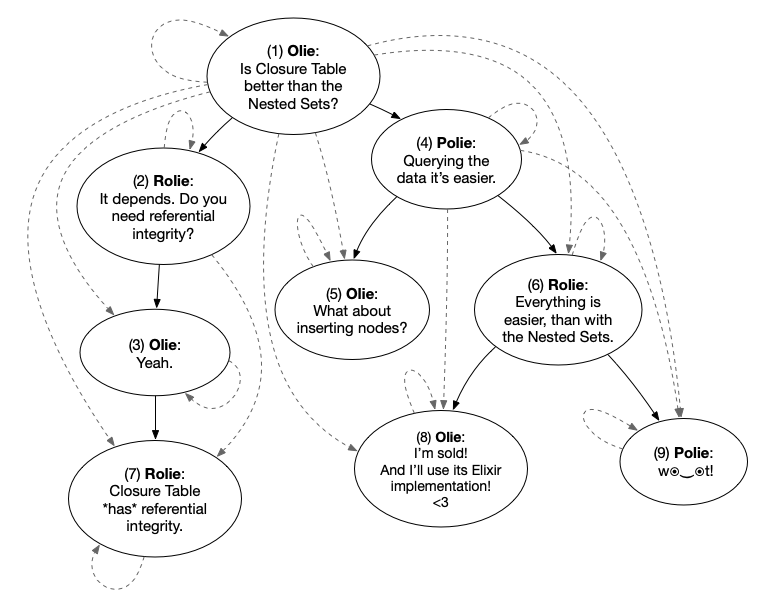
\includegraphics[width=\textwidth]{closure_table}
    \end{figure}
    
    Esta solución es la más versátil y rápida de todas las mostradas en [], permitiendo incluso a un nodo pertenecer a varios árboles. Sin embargo, estos beneficios los consigue a costa de espacio. Este consumo puede ser importante si la estructura almacena jerarquías muy profundas.
    \\
    
    No obstante todo lo discutido con anterioridad, la solución real implementada para el trato específico de las categorías es triple: Closure table, lista de adyacencia y trabajo en memoria principal con una estructura de datos en árbol. Esto es así por una cuestión de eficiencia y por desarrollar experiencia en el uso de estas soluciones.
    \\
    
    \begin{lstlisting}[caption=Tablas que gestionan las categorías]
    create table category (
    	id bigint not null, 
    	created_by varchar(255), 
    	created_date timestamp, 
    	last_modified_by varchar(255), 
    	last_modified_date timestamp, 
    	name varchar(255), 
    	parent_id bigint, 
    	primary key (id)
    );
    	
    create table catpath (
    	id bigint not null, 
    	created_by varchar(255), 
    	created_date timestamp, 
    	last_modified_by varchar(255), 
    	last_modified_date timestamp, 
    	size integer not null, 
    	ancestor_id bigint, 
    	descendant_id bigint, 
    	primary key (id)
    );
    
    alter table category 
    	add constraint fk_parentIdOnCategory foreign key (parent_id) references category(id)
    ;
    
    alter table catpath 
    	add constraint fk_ancestorIdOnCatpath foreign key (ancestor_id) references category(id)
    ;
    
    alter table catpath 
    	add constraint fk_descendantIdOnCatpath foreign key (descendant_id) references category(id)
    ;
    
    
    \end{lstlisting}
    
    \subsection{Validación}
    Por validación se entiende las comprobaciones que la aplicación web hace sobre los datos que le son proporcionados externamente. El caso más común es cuando un usuario envía un formulario cumplimentado a la aplicación web, y esta, antes de procesar la información, comprueba que se cumplen ciertas reglas. Por ejemplo, puede requerirse que el campo de email sea efectivamente una dirección de correo válida, o que la fecha de nacimiento sea una fecha pasada válida (nadie puede nacer el 30 de febrero, por ejemplo). Esto se hace para garantizar la consistencia de los datos en la base de datos y por motivos de seguridad, como evitar ataques de inyección SQL.
    \\
    
    Esta comprobación se puede hacer tanto en cliente como en servidor. Desde el punto de vista de la seguridad, realizar la comprobación en servidor es obligatorio, ya que las comprobaciones en cliente son muy fácilmente circunvaladas. Por otro lado, desde el punto de vista de la experiencia de usuario es muy recomendable implemetarla también en cliente, ya que permite al usuario tener un feedback mucho más rápido que si debiese esperar a que el servidor responda. En definitiva, la mejor práctica es implemetar la validación tanto en backend como en frontend. Y así se ha hecho.
    \\
    
    Mucha es la información que FirstMarket tiene que validar, pero a grandes rasgos se puede dividir en numérica y textual. El primer grupo presenta poca dificultad, se trata de comprobar rangos de valores principalmente. Para el segundo grupo las expresiones regulares son el arma perfecta. En el archivo de configuración \emph{application.yml} se detallan las expresiones regulares y los rangos numéricos utilizados. A modo de ejemplo, la propiedad definida en este archivo de configuración que especifica la expresión regular contra la que comparar las contraseñas es la siguiente:
    \\
     
    \begin{lstlisting}[caption=Expresión regular para las contraseñas]
    fm:
      validation:
        regex:
          password: ^(?=.*\d)(?=.*[a-z])(?=.*[A-Z]).{8,16}$
    \end{lstlisting}
    
    Así, esta expresión regular es utilizada por la aplicación web para comprobar, tanto en frontend como en backend, que cuando un usuario proporciona una nueva contraseña esta tenga una longitud de entre 8 y 16 caractéres e incluya al menos una minúscula, una mayúscula y un dígito.
    \\
    
    Sin embargo, existe un campo que destaca por su manera de ser validado. Se trata del ISBN (International Standard Book Number) de los libros. Este campo necesita validación en dos vertientes, a saber, sintáctica y semántica. La validación sintáctica se realiza utilizando las ya mencionadas expresiones regulares, pero para validar si se trata de un ISBN válido aún hay que calcular mediante un algoritmo concreto un dígito de control y ver si el último dígito coincide. Los ISBN tuvieron 10 dígitos hasta diciembre de 2006 pero, desde enero de 2007, tienen siempre 13 dígitos (ambas versiones con diferentes algoritmos de cálculo de dígito de control). Así pues, la validación debe dar soporte a ambos formatos de ISBN. A modo de ejemplo se detalla a continuación la función en JavaScript desarrollada para comprobar en el cliente el dígito de control:
    \\
    
    \begin{lstlisting}[language=JavaScript,caption=Validación del dígito de control del ISBN en cliente]
    const isbnChecksum = function() {
    	let chars, last, sum, check, i;
    	const isbn = document.getElementById("isbn");
    	if (isbn.checkValidity()) {
    		// Remove non ISBN digits, then split into an array
    		chars = isbn.value.replace(/[- ]|^ISBN(?:-1[03])?:?/g, "").split("");
    		// Remove the final ISBN digit from `chars`, and assign it to `last`
    		last = chars.pop();
    		sum = 0;
    		if (chars.length == 9) {
    			// Compute the ISBN-10 check digit
    			chars.reverse();
    			for (i = 0; i < chars.length; i++) {
    				sum += (i + 2) * parseInt(chars[i], 10);
    			}
    			check = 11 - (sum % 11);
    			if (check == 10) {
    				check = "X";
    			} else if (check == 11) {
    				check = "0";
    			}
    		} else {
    			// Compute the ISBN-13 check digit
    			for (i = 0; i < chars.length; i++) {
    				sum += (i % 2 * 2 + 1) * parseInt(chars[i], 10);
    			}
    			check = 10 - (sum % 10);
    			if (check == 10) {
    				check = "0";
    			}
    		}
    		if (check != last) {
    			alert("Error: Invalid ISBN checksum digit (" + last + "). Try with (" + check + ")");
    			isbn.focus();
    			isbn.value = isbn.value.substring(0, isbn.value.length - 1);
    		}
    	}
    };
    \end{lstlisting}
    
    
    
    
    

    % TECNOLOGIAS
    \section{Stack Tecnológico}
    En este apartado se ofrece un comentario del stack tecnologico con el que se ha llevado a cabo la aplicacion web.

    \subsection{Spring Framework}
    \subsubsection{Spring Boot}
    \subsubsection{Spring MVC}
    \subsubsection{Spring Data JPA - Hibernate}
    \subsubsection{Spring Security}
    \subsection{Thymeleaf - HTML5}
    \subsection{Bootstrap 4 - CSS3}
    \subsection{Stripe}
    \subsection{PostgreSQL}
    \subsection{JavaScript}
    \subsubsection{Ajax}
    \subsection{FontAwesome - Pretty Checkbox - Google Fonts}
    \subsection{Tecnologias Transversales}
    \subsubsection{Git}
    \subsubsection{Java 11}
    \subsubsection{Maven}
    \subsubsection{IntelliJ IDEA}
    \subsubsection{Logback}
    \subsubsection{Lombok}
    \subsubsection{Guava}

    % DESPLIEGUE Y SEGURIDAD
    \section{Despliegue y Seguridad}
        \subsection{Heroku Platform}
            \subsubsection{Heroku-postgresql}
            \subsubsection{PaperTrail}
            \subsubsection{Snyk}
        \subsection{Spring Security}
        \subsection{HTTPS}
        \subsection{Cross-Site Request Forgery}
        \subsection{Brute-Force Authentication}

    % MANUALES
    \section{Manuales}
    En esta seccion se va a describir las cuestiones necesarias para facilitar el uso de la aplicacion web por parte de los usuarios
        \subsection{Usuario Cliente}
    aqui va la descripcion para el usuario cliente
        \subsection{Usuario Administrador}
    aquie se describe el uso del admin

	% PRESUPUESTO
	\section{Presupuesto}

    % MEJORAS Y AMPLIACIONES
    \section{Mejoras y Ampliaciones}
    Testar el software
    Sistema de valoracion por parte de los usuarios de los libros


\end{document}
